\documentclass[11pt,letterpaper]{article}
\usepackage[utf8]{inputenc}
\usepackage[T1]{fontenc}
\usepackage[margin=1in]{geometry}
\usepackage{amsmath,amssymb}
\usepackage{graphicx}
\usepackage{hyperref}
\usepackage{xcolor}
\usepackage{enumitem}
\usepackage{caption}

\hypersetup{colorlinks=true,linkcolor=black,urlcolor=black,citecolor=black}
\graphicspath{{../figures/}}

\title{\textbf{\$ZOO Tokenomics}\\\large Gold/Silver-Backed Native Token, Bridges, Liquidity, and Sustainability Tax}
\author{Antje Worring \\ \textit{Founder, Zoo Labs Foundation} \\ \texttt{antje@zoo.ngo}}
\date{October 31, 2021}

\begin{document}
\maketitle

\begin{abstract}
This element paper extracts the tokenomics from the Zoo Whitepaper~\cite{zoo2021}: \$ZOO as the native token backed by gold and silver via Lux Tokens, the bridge protocol that delivers cross-chain mobility, the liquidity-protocol design that makes every NFT an LP position, and the sustainability tax that routes value to the DAO and liquidity pool.
\end{abstract}

\section{\$ZOO: a commodity-backed native token}

\$ZOO sits at the centre of the Zoo ecosystem. Its distinguishing feature is its backing: the largest liquidity pools contain Lux Tokens, which are themselves backed by silver and gold. This backing transfers tangible commodity value into the digital ecosystem, providing stability and a real-world value anchor.

Token holders may transfer, sell, or redeem Lux Tokens for their physical counterparts. The initial commodity scope is precious metals; future expansions broaden to other natural resources.

\section{The bridge protocol}

The Zoo Bridge eliminates vault custody. Instead of trapping tokens in a vault contract, the bridge:

\begin{enumerate}
  \item Burns \$ZOO on the source chain.
  \item Has MPC validators verify the burn via threshold signatures (TSS).
  \item Mints \$ZOO on the destination chain when two-thirds of validators sign.
\end{enumerate}

The validator network is leaderless. Each validator runs the same process on receipt of on-chain events from any of the chains the MPC group tracks. Standard transactions wait for three network confirmations before mint.

This burn-and-mint design avoids the vault-vulnerability class of bridge exploit that has dominated cross-chain hacks.

\section{NFT-as-LP: the liquidity protocol}

Zoo is a liquidity protocol for NFTs in the way Uniswap is for tokens. The core mechanic:

\begin{itemize}
  \item Adding collateral to an NFT is providing liquidity.
  \item Burning the NFT redeems the underlying assets (collateral + rewards) like burning an LP token.
  \item Pools allow listing two or more NFTs at a chosen aggregate price for a single-purchase transfer.
\end{itemize}

Every NFT is therefore a user-defined liquidity position. The intrinsic value floor is the staked collateral. The market value can be higher (rarity premium) or, in extreme conditions, lower (rarity discount).

\section{Sustainability tax}

The whitepaper specifies several tax flows:

\begin{itemize}
  \item \textbf{Burn tax.} 20\% of the burn refund: 10\% to the DAO conservation treasury, 10\% to the liquidity pool.
  \item \textbf{Transaction tax.} 4\% to the DAO, 4\% to liquidity, on the broader transaction set described in the Metaverse Companion section.
  \item \textbf{Breeding fee.} 3$\times$ the original egg price for adult-adult breeding flows to the DAO.
\end{itemize}

These flows together keep the liquidity pool deep, fund the conservation treasury, and reward the DAO operationally.

\section{Reward economics}

\paragraph{Initial allocation.} 50\% of the entire token supply is allocated to rewards at the Gen 0 drop.

\paragraph{Reward duration.} Daily rewards on each Gen 0 animal continue for two years after the animal is minted.

\paragraph{Boost amplification.} Collateral staked into the NFT amplifies the daily reward via a 1.1$\times$--1.4$\times$ boost ladder, keyed to dollar value of collateral.

\paragraph{DAO governance.} Future reward modifications, extension of the reward period, or new reward streams are subject to the Zoo DAO's governance process.

\section{The unified picture}

\$ZOO's value derives from four anchors:

\begin{enumerate}
  \item \textbf{Commodity backing} via Lux Tokens.
  \item \textbf{NFT collateral} locked across the ecosystem.
  \item \textbf{Buy pressure} from gameplay (mint costs, breeding fees).
  \item \textbf{Tax-driven liquidity replenishment} (the 4\%/4\%/burn-tax flows).
\end{enumerate}

These anchors compound. As more animals are minted, more collateral locks. As more transactions execute, more tax flows to liquidity. As the conservation treasury grows, the DAO's mission deepens. The architecture is designed to be cycle-resistant.

\begin{figure}[h]
\centering
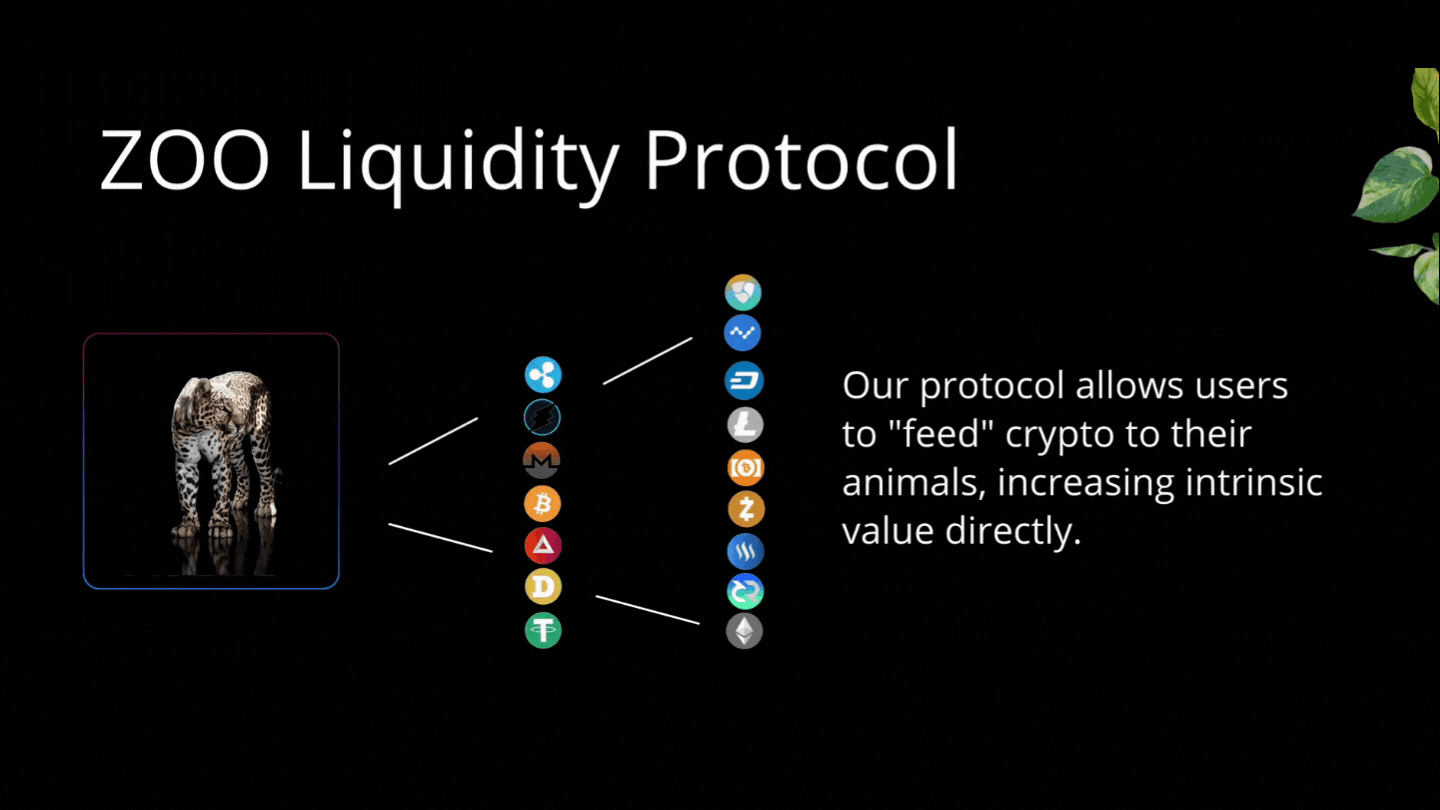
\includegraphics[width=0.6\textwidth]{liquidity-protocol.png}
\caption{Liquidity protocol diagram. Each NFT is itself a liquidity-pool position: collateral is added by feeding, withdrawn by burning. The protocol routes tax across the LP, the DAO, and the conservation treasury.}
\end{figure}

\section{The KEEPER token}

Alongside \$ZOO, the Zoo DAO mints \textbf{KEEPER} as a governance token. KEEPER is earned by completing quests and contributing to the community. Holders ``bet'' on proposals rather than vote in a binary fashion; winning bets yield additional KEEPER, promoting active participation. KEEPER is subject to the same 8\% liquidity-pool tax (4\% LP, 4\% DAO) as \$ZOO on every sell, ensuring the DAO treasury grows alongside KEEPER's circulating supply.

\section{Treasury management}

The whitepaper~\cite{zoo2021} specifies that \emph{half} of the \$ZOO supply is reserved within the Treasury. This allocation:

\begin{itemize}
  \item Funds the daily-reward stream for two years post-mint per Gen 0 animal.
  \item Maintains buffer liquidity through market cycles.
  \item Provides DAO-controlled discretionary funds for partnership, education, and conservation initiatives.
\end{itemize}

The Treasury is not a slush fund. Disbursements are governed by DAO vote and recorded on chain.

\section{Validator economics}

A Lux Layer-1 validator allocated to the Zoo protocol generates transaction fees within the Lux network. Those fees provide a continual influx of liquidity to the Zoo Treasury, decoupled from secondary-market volatility. This validator-driven liquidity is what makes the long-term reward distribution sustainable beyond the initial 50\% allocation.

\section{Bridge protocol details}

The Zoo Bridge Protocol~\cite{zoo2021} merits more depth because the standard \emph{lock-in-vault} bridge design has been the source of the largest cross-chain hacks. The Zoo Bridge instead:

\begin{itemize}
  \item Uses MPC validators with threshold signature schemes (TSS) rather than a custodial vault contract.
  \item Achieves consensus when 2/3 of all validators sign the same transaction.
  \item Burns on the source chain, mints on the destination, never holding tokens in a single contract that can be drained.
  \item Waits for 3 network confirmations on the source chain before allowing mint --- a deliberate latency-versus-safety choice.
\end{itemize}

The bridge enables \$ZOO to move between Binance Smart Chain (initial deployment), Ethereum, and any chain with sufficient validator coverage. This is what makes Zoo's user acquisition multi-chain rather than single-chain.

\begin{figure}[h]
\centering
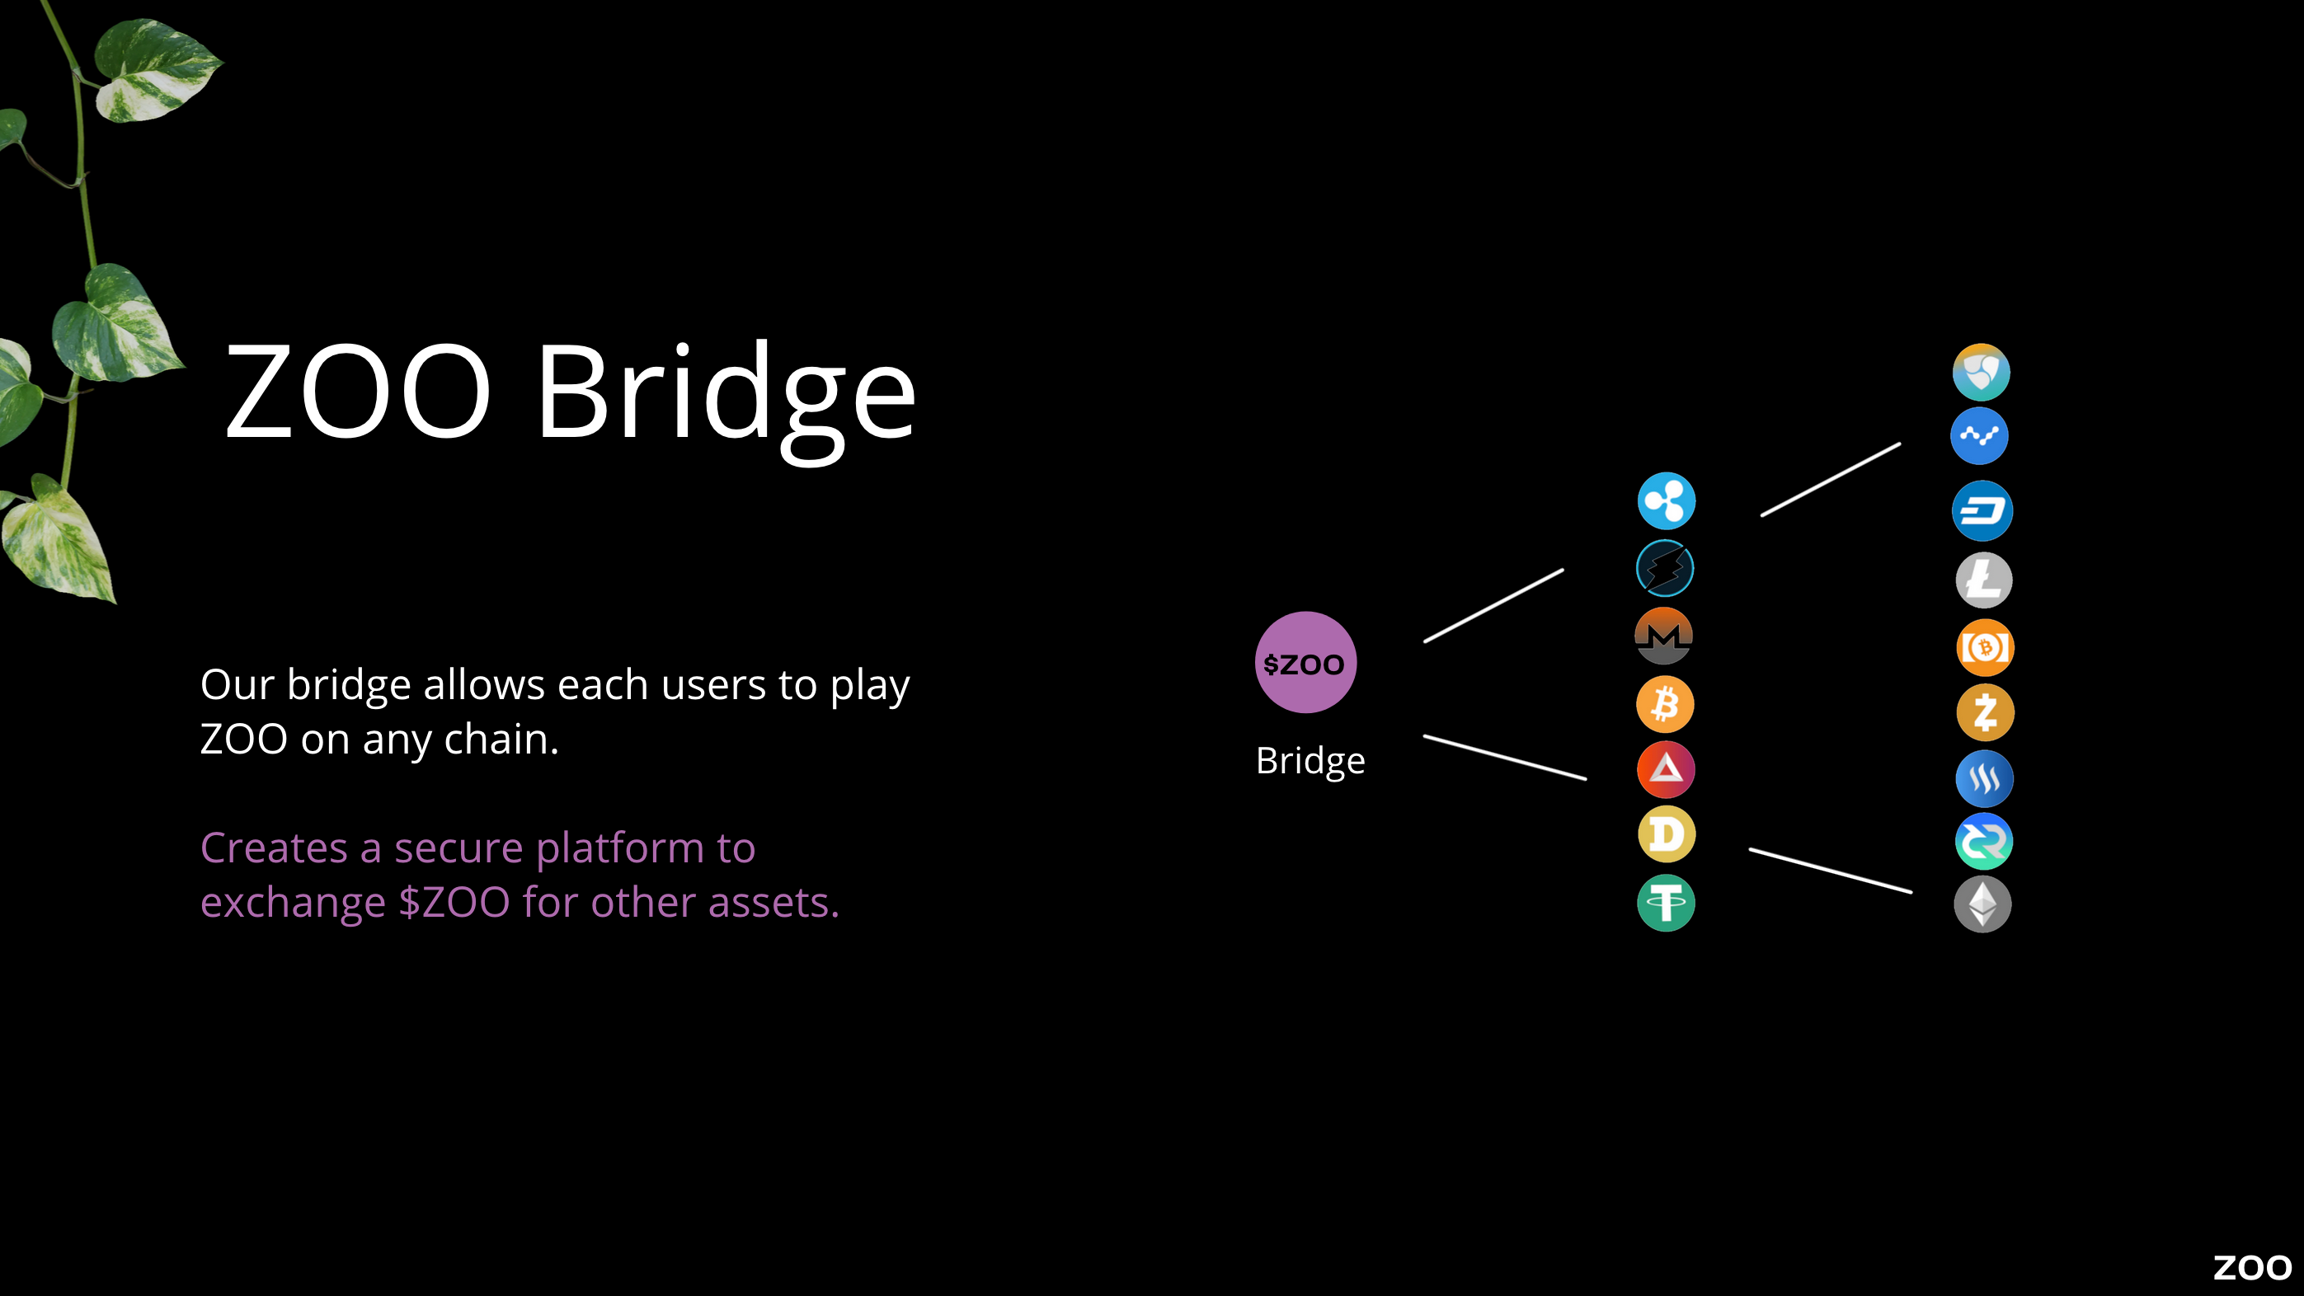
\includegraphics[width=0.6\textwidth]{bridge.png}
\caption{Zoo Bridge architecture. MPC validators monitor on-chain events across chains. Threshold signatures gate the burn-and-mint transition without ever holding tokens in a vault contract.}
\end{figure}

\begin{thebibliography}{1}
\bibitem{zoo2021} Antje Worring. \emph{Zoo: A Game-Fi Multiverse Ecosystem for the Preservation of Endangered Species}. Zoo Labs Foundation, October 31, 2021.
\end{thebibliography}

\end{document}
